% can't include for some reason... must be input
\pagebreak
\subsection{run\_AGC\_mod - WIP} \label{ex: agc mod}
An extended term simulation may required the adjustment of scheduled interchange to achieve system recovery.
Specifically, if an area realizes that their available reserves become lower than was originally allocated for, a resolution may be to import more power from another area.
Functionality to accomplish such a task was added via a user defined \verb|mAGC_sig| fuction.
Similar to other \verb|m*_sig| files, it is executed every time step and allows for setting an area's \verb|icAdj| value to any value.


The \verb|run_AGC_mod| example adjusts the interchange modulation signal as a perturbance and allows AGC to re-balance line flows accordingly.
As a reminder, the one-line diagram of the system used is shown in Figure \ref{fig: runAGC one line}.
%Sloppily copied from: \verb|200821-AGCicAdjTest|
When $t=5$, Area 2 increased scheduled interchange by 0.2 PU while Area 1 interchange is adjusted by -0.2 PU to keep system in balance.
Each area has non-conditional AGC set to act every 15 seconds and is forced to act by user defined code in \verb|mAGC_sig| when the interchange adjustment first takes place.
The example showed how Area 2 increased generation while Area 1 reduced generation in response to the interchange modulation signal.

%\item ODE solver tolerances:
%\subitem Relative: 1e-5
%\subitem Absolute: 1e-7

\subsubsection{run\_AGC\_mod Result Summary - WIP}
Interchange adjustment worked as expected and was accounted for in AGC calculations.
The use of \verb|mAGC_sig| was tested as working using FTS or VTS.
The \verb|mAGC_sig| file used to adjust interchange and force AGC action is shown as Listing \ref{lst: agc mod def}.


\begin{figure}[H]
	\centering
	\footnotesize
	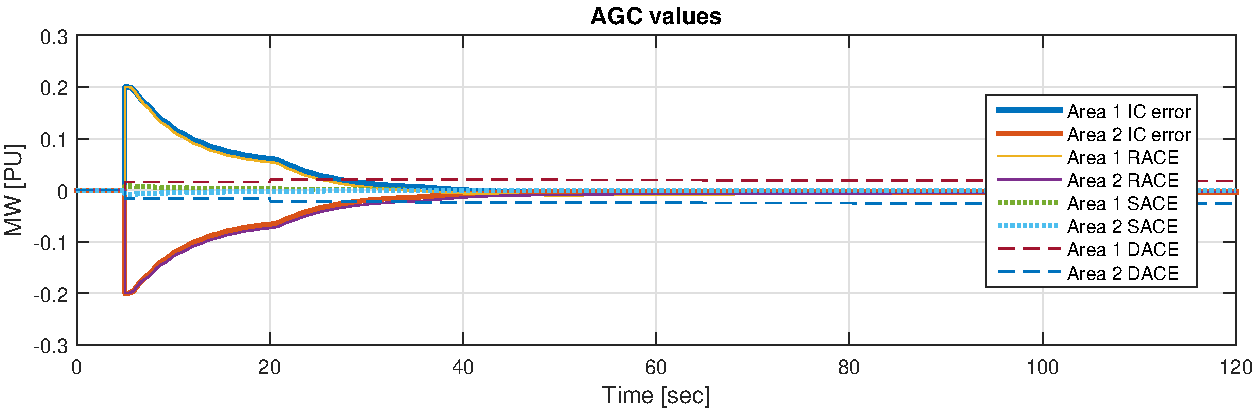
\includegraphics[width=\linewidth]{examples/agcMod/agcModSig01}
	\caption{AGC signals from run\_AGC\_mod example.}
	\label{fig: AGCmod liveplot}
\end{figure}%\vspace{-1 em}

\begin{figure}[H]
	\centering
	\footnotesize
	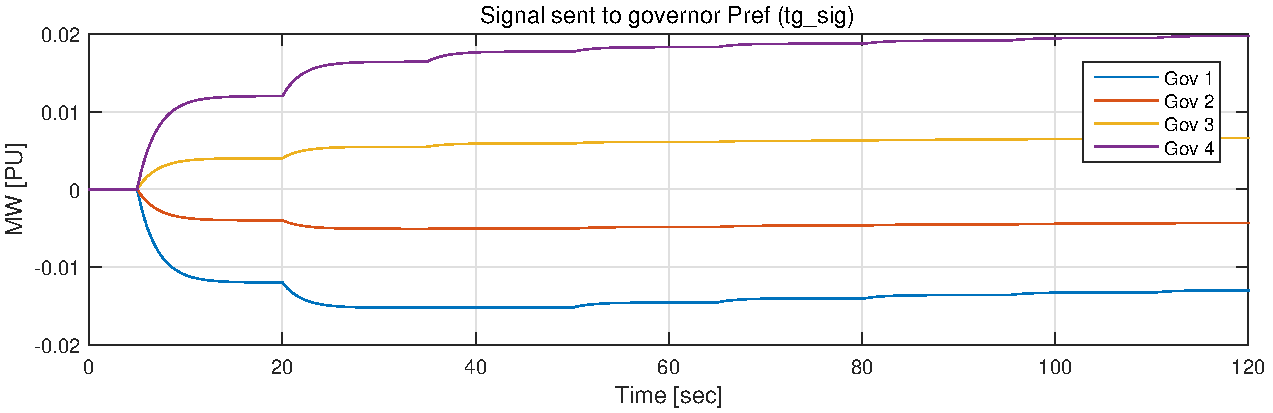
\includegraphics[width=\linewidth]{examples/agcMod/agcModSig02}
	\caption{Turbine governor modulation signals from run\_AGC\_mod.}
	\label{fig: AGCmod tg sig}
\end{figure}%\vspace{-1 em}

\begin{figure}[H]
	\centering
	\footnotesize
	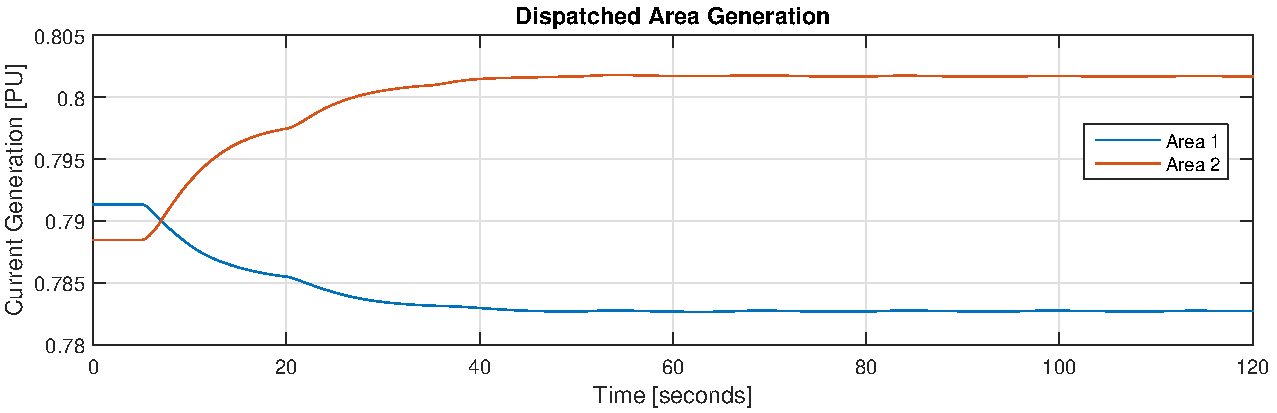
\includegraphics[width=\linewidth]{examples/agcMod/agcModSig03}
	\caption{Change of dispatched area generation during run\_AGC\_mod.}
	\label{fig: AGCmod area gen}
\end{figure}%\vspace{-1 em}

\begin{figure}[H]
	\centering
	\footnotesize
	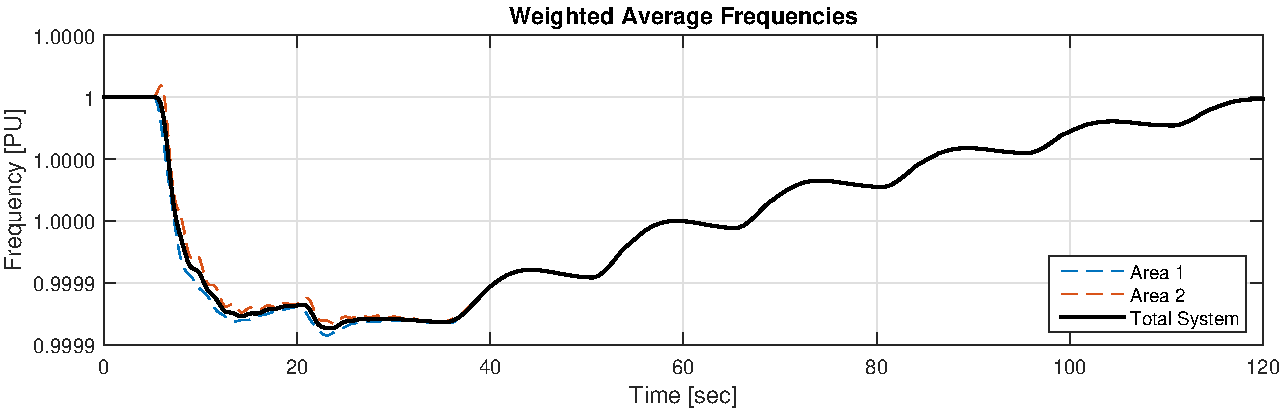
\includegraphics[width=\linewidth]{examples/agcMod/agcModSig04}
	\caption{Change in system frequency during run\_AGC\_mod.}
	\label{fig: AGCmod change in gen}
\end{figure}%\vspace{-1 em}

\pagebreak


\begin{lstlisting}[caption={AGC Modulation Example},label={lst: agc mod def}]
\end{lstlisting}\vspace{-2 em}
\begin{minted}[
		frame=lines,
		framesep=2mm,
		baselinestretch=1.2,
		bgcolor=gray!13,
		fontsize=\footnotesize,
		linenos,
		breaklines
		]{MATLAB}
function mAGC_sig(k)
% Syntax: mAGC_sig(k)
% input k is current data index
% 09:46 08/21/20
% place to define modulation signal for AGC operation

global g

%{
    Scenario:
Area 1 is exporting generation to Area 2 (Interchange value Positive)
Area 2 is importing power from Area 1 (Interchange value is Negative

Area 2 increases scheduled interchage, which reduces its scheduled import and causes area 2 to increase generation.
Area 1 decreases scheduled interchange to balance area 2 action.
As area 1 is exporting, the negative valued icAdj will reduce the generation in the area.
%}
persistent ForceDisptach

if g.sys.t(k) >= 5
    % adjust iterchange 
    g.area.area(2).icAdj(k) = 0.2;
    g.area.area(1).icAdj(k) = -0.2;
    
    % force AGC disptatch when interchange adjustment first applied
    if ForceDisptach
        g.agc.agc(1).nextActionTime = g.sys.t(k);
        g.agc.agc(2).nextActionTime = g.sys.t(k);
        ForceDisptach = 0;
    end 
else
    g.area.area(2).icAdj(k) = 0;
    g.area.area(1).icAdj(k) = 0;
    ForceDisptach = 1;
end
end
\end{minted}
